\chapter{recommendation for further work regarding the full system}

	Furthemore, a framework to test and build an entire automated system is suggested. This framework includes a 
	simulated envorinment, that realisicly makes it possible, to navigate a drone within an simulated environment. The environment 
	is based on the Roboter Operating System (ROS) and is completely simulated. 
	
	The basic idea of the framework can be seen in figure \ref{fig:autsys}. The main parts of the automated exploration system are the SLAM Algorithm
	and the flight path planning algorithm, that work simultaniously. The general concept is that each of the algorithms takes the output of the other as 
	input. 
	
	In the folling section the ROS framework is proposed and described in detail. 
	
	\fig{img/aut_system.png}{Automated SLAM system}{fig:autsys}{0.8}


\section{ROS framework}

		
	ROS, as the name suggests, is a framework for a software infrastracture within a robot. With the right drivers installed, 
	it can access and use the robots hardware and serves as a messenger system between robot components. Ros packages make it easy to 
	reuse important functionalities. Gazebo on the other hand is a 3D dynamic simulator for robotics. It can accurately and efficiently simulate robots regarding
	their physics. 
	
	\fig{img/aut_ros.png}{Overview over the suggested ROS framework}{fig:autros}{0.95}
	
	% Sprachenunabhängig
	
	\subsection{TUM Simulation Node}
	
	Thus, with the tum\_simulation package you can navigate an AR.drone 1.0 and 2.0 in different worlds created with a gazebo node. This drone is eqipped with a bottom camera 
	and a frot camera. The cameras each log their output to a ros topic. Additionally, message time stamps, the height sensor output, 
	battery percentage, rotation
	velocity and accelaration are also logged to rostopics. While the drone can also be navigated using a playstation 3 controller, as shown in figure 
	\ref{fig:tumsim}, showing a section of the tum\_simulation package content structure, 
	for an automated system, the drone should rather be addressed using the command line interface. For example 
	the command shown in sourcecode listing \ref{lst:drone_cmd} will make the drone fly foreward. 
	
	\begin{lstlisting}[language=bash, caption=drone navigation command, label=lst:drone_cmd]
    rostopic pub -r 10 /cmd_vel geometry_msgs/Twist  '{linear:  {x: 1.0, y: 0.0, z: 0.0}, angular: {x: 0.0,y: 0.0,z: 0.0}}'
	\end{lstlisting}
	
	\fig{img/tum_sim.png}{tum simulator setup. Source: $http://wiki.ros.org/tum_simulator$}{fig:tumsim}{0.8}
	
	
	In figure \cite{fig:simfigs} the simulated environment with gazebo can be found in figure a. Here, the drone (in black) is flying in front of the building. 
	The output of the front camera is shown in figure b. Therefore, the output calibration data of the front camera, such as the focal lengt, 
	can be found in an own rostopic. In figure c, the ORB-SLAM-Algorithm was applied to the output of the front camera. Green dots represent the 
	finding of an ORB-feature. 
	
	\subsection{ORB-SLAM Node}
	
	The ORB-SLAM algorithm runs in 
	
	\subsubsection{Input}
	\subsubsection{Output}
	
	\subsection{Position Estimation Node}
	
	The position estimation node appriximates the position of the drone based on the valocity on the drone and the latest position. ORB-SLAM, used 
	in the visual monocular mode is as mentioned not able to extract the true scale of the environment. Estimating the true position enables us 
	to also scale the computed point cloud by the ORB SLAM node to its true scale. This method should be done in the initialization process, by 
	only doing translational movements with the drone, such as a takeoff and a short foreward movement. No rotations should be performed with the drone 
	since the drones navigation data, such as the veloxity, uses the bodyframe as reference frame. Thus doing rotations would result in an incorrect 
	estimation of the position. While relying on the information about the 
	velocity of the drone, the drone needs to have inertial sensors attached. Having these IMU sensors, as the ardrone in the simulation does, also ORB SLAM would benifit from 
	accuracy, since it the integration in the algorithm is implemented. However, if drone does not have these sensors attached, 
	this node can still be of benefit, since it is possible to manually publish messanges to the topic. The initialization process could then be applied 
	by manually flying the drone one meter up, and one meter foreward and logging these points to the system. Then the automazation process could be started.
	Folling an overview over the input, output and computational functionality of the node. 
	
	\subsubsection{Input}
	
	The node subscribes to the following topics:
	
	\begin{enumerate}
	\item{/ardrone/navdata}
	
	This topic is beeing published with the tum simulation node described in item \ref{asdfasdf} and is a messenger class developed for the ardrone.
	This node only uses the velocity vectors
	$v_x \in \mathbb{R}, v_y \in \mathbb{R}, v_z \in \mathbb{R}$ given in the unit $mms^{-1}$. 
	
	\item{/drone\_position\_init}
	
	The drone also subscribes to the /drone\_position\_init topic, published by itself. This topic includes messenges of the class PointStamped. 
	This class includes the x, y and z coordinate of the point itself, and a timestamp.  
	The node also needs the information from this topic, 
	to read in the last position and update it based on the velocity, by doing the computations explained in the following section. The x y and z 
	coordinates are transformed to meter. 
	\end{enumerate}
	
	\subsubsection{Output}
	
	The node publishes to the following topics:
	
	\begin{enumerate}
	\item{/drone\_position\_init}
	
	This topic is explained in the upper section. The updated points are published in this topic
	
	\end{enumerate}
	
	\subsubsection{computation}
	
	As mentioned, the computation is made based on the current velocity $$v_i = \begin{pmatrix} v_{i,x} \\ v_{i,y} \\ v_{i,z} \end{pmatrix} \in \mathbb{R}^3$$ and the 
	latest position point $$x_{i-1} = \begin{pmatrix} x_{i-1,x} \\ x_{i-1,y} \\ x_{i-1, z} \end{pmatrix} \in \mathbb{R}^3$$. Also, the timedifference 
	in seconds to the last point is extracted, which is easy, since all onject from the class PointStamped can be timestamped. The difference is given by 
	$\Delta t_i =  t_i - t_{i-1}$. The updated position is the yielded by
	
	$$x_{i} = x_{i-1} + \frac{\Delta t_i * v_i}{1000} $$. 
	
	Dividing by 1000 yields the unit meter. 
	
	This recursive methodoly is shown in figure \ref{fig:positionfinding}
	
	\fig{img/pos_estimation.png}{Calculation method for estimation the position in the initialization porcess in order to find the 
	true scale.}{fig:positionfinding}{0.8}
	
	The implementation is easily deployed and the update function, that is running in the main loop can be seen in listing \ref{lst:posupdate}. 
	
	\begin{lstlisting}[language=python, caption=Main part of the position estimation node, label=lst:posupdate]
	def update_position(self):
        # get velocity in x, y and z direction
        x_vel = self.navdata.vz
        y_vel = self.navdata.vy
        z_vel = self.navdata.vz

        if x_vel is not None and y_vel is not None and z_vel is not None:
			# get time difference
            curr_time = rospy.Time.now()
            time_diff = (curr_time - self.position.header.stamp).to_sec()
			
			# create the new point
            new_point = PointStamped()
            new_point.header.stamp = curr_time
            new_point.header.frame_id = "init"
			
			# update positions
            new_point.point.x = self.position.point.x + time_diff * x_vel / 1000
            new_point.point.y = self.position.point.y + time_diff * y_vel / 1000
            new_point.point.z = self.position.point.z + time_diff * z_vel / 1000
			
			# publish
            self.position_publisher.publish(new_point)
            rospy.sleep(0.1)
	\end{lstlisting}
	
	\subsection{Scale Recognition Node}
	
	This node estimates the true scale of the pointcloud. This is beneficial to later use the pointcloud for real life purposes. 
	This is done by aligning the estimated position based on the velocity of the drone in the initialization process and the 
	estimated position of the drone by the ORB-SLAM Algorithm. 
	
	\subsubsection{Input}
	\subsubsection{Output}
	\subsubsection{computation}
	
	
	\begin{lstlisting}[language=python, caption=Main part of the scale estimation node, label=lst:scaleup]
def update_scale(self):
# return, if not enough points are available
# since no scale can be computed
if (len(self.est_pos_orb) < 25) or (len(self.est_pos_vel) < 25):
	return

# return the scale if it already has been calculated    
elif self.scale:
	return
else:
	# get minimum and maximum time for each queue to figure out, 
	# how many points can be considered for alignment. This is only done once!
	min_orb = np.min([pose_oi.header.stamp.to_sec() for pose_oi in self.est_pos_orb])
	max_orb = np.max([pose_oi.header.stamp.to_sec() for pose_oi in self.est_pos_orb])

	min_vel = np.min([point_oi.header.stamp.to_sec() for point_oi in self.est_pos_vel])
	max_vel = np.max([point_oi.header.stamp.to_sec() for point_oi in self.est_pos_vel])

	thresh_min = np.max([min_orb, min_vel])
	thresh_max = np.min([max_vel, max_orb])

	# cut off the queues
	orb_oi = [pose_oi for pose_oi in self.est_pos_orb if pose_oi.header.stamp.to_sec() > thresh_min]
	vel_oi = [point_oi for point_oi in self.est_pos_vel if point_oi.header.stamp.to_sec() > thresh_min]

	# for the shorter remaining queue, get the matching point
	if len(orb_oi) <= len(vel_oi): 
		orb_oi_final = orb_oi
		vel_oi_final = []
		for pose_oi in orb_oi: 
			diffs_oi = [np.abs(pose_oi.header.stamp.to_sec() - point_oi.header.stamp.to_sec()) for point_oi in vel_oi]
			vel_oi_final.append(vel_oi[diffs_oi.index(min(diffs_oi))])

	else:
		vel_oi_final = vel_oi
		orb_oi_final = []
		for pose_oi in vel_oi: 
			diffs_oi = [np.abs(pose_oi.header.stamp.to_sec() - point_oi.header.stamp.to_sec()) for point_oi in orb_oi]
			vel_oi_final.append(vel_oi[diffs_oi.index(min(diffs_oi))])


	# now do the alignment and compute the scale
	x_orb = [pose_oi.pose.position.x for pose_oi in orb_oi_final]
	y_orb = [pose_oi.pose.position.y for pose_oi in orb_oi_final]
	z_orb = [pose_oi.pose.position.z for pose_oi in orb_oi_final]

	x_vel = [point_oi.point.x for point_oi in vel_oi_final]
	y_vel = [point_oi.point.y for point_oi in vel_oi_final]
	z_vel = [point_oi.point.z for point_oi in vel_oi_final]
	
	orb_points = np.column_stack((x_orb, y_orb, z_orb))
	vel_points = np.column_stack((x_vel, y_vel, z_vel))

	s, R, t = align_umeyama(vel_points, orb_points)

	# finally publish the computed scale 
	self.scale_publisher.publish(Float64(s))
	self.scale = s
	\end{lstlisting}
	
	\subsection{Fight Path Planning Node}
	
	\subsubsection{Input}
	\subsubsection{Output}
	
	\section{Current setup}
	
	\begin{figure}%
    \centering
    \subfloat[\centering gazebo simulation]{{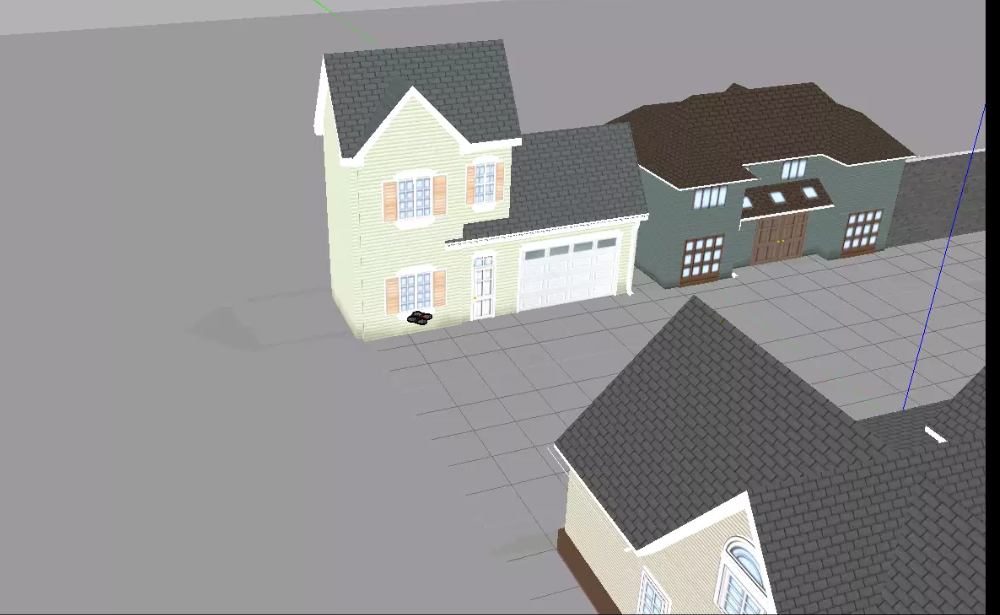
\includegraphics[width=5cm]{img/drohne_oben.png} }}%
    \qquad
    \subfloat[\centering front camera simulation]{{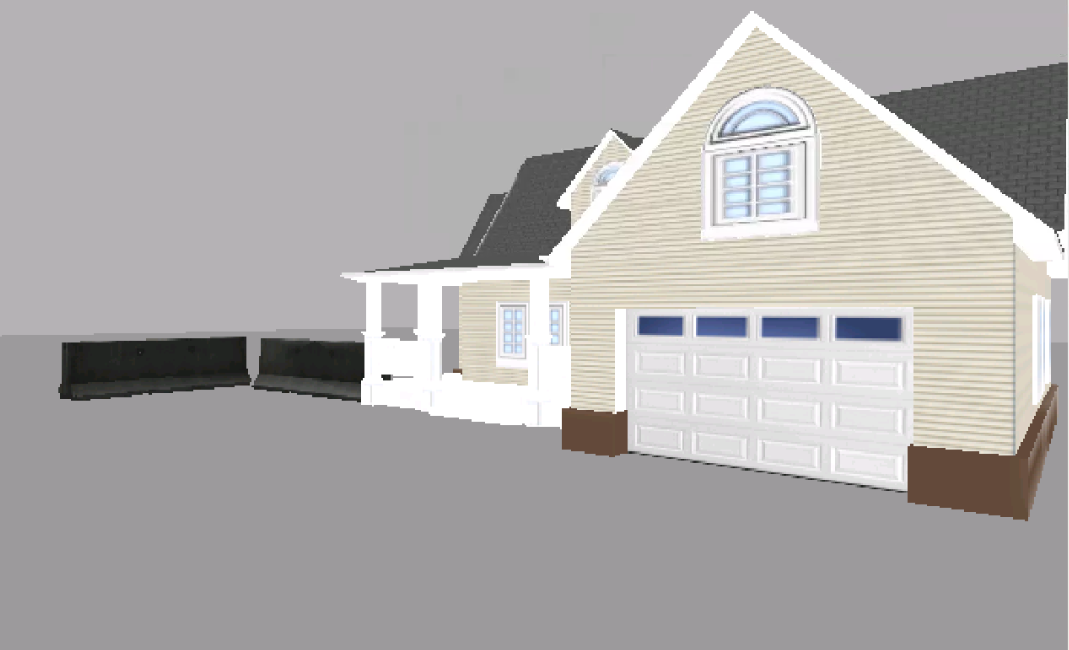
\includegraphics[width=5cm]{img/drohne_kamera.png} }}%
	\qquad
    \subfloat[\centering ORB applied on simulation]{{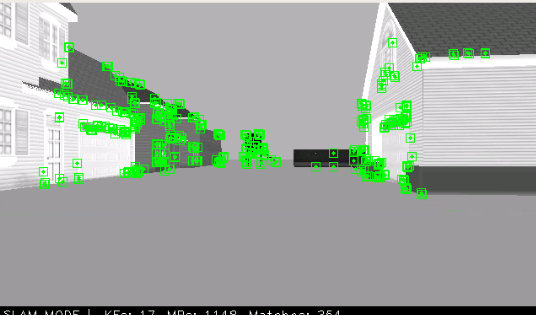
\includegraphics[width=5cm]{img/front_camera_orb.png} }}%
    \caption{
	The drone in a gazebo simulation in a), the output of the front camera of the drone in b) and
	the ORB-SLAM algorithm applied on the front camera output in with the detected ORB features marked green c).
	}%
    \label{fig:simfigs}%
	\end{figure}
	
	Currently the framework is set up in an environment provided by theconstructsim.com. This platform is enabling ROS-developers to program in preconfigured
	ROS-environments. The environment comes with the possibility to open terminal consols, a file management system, a simulator, that automatically 
	detects, when a gazebo simulation is running. Also, you have a graphical interface for other graphical applications, such as the viewer of ORB-SLAM.
	The current environments is set up with ROS kinetic and Ubuntu 16.04.6 LTS (Xenial). The tum\_simulator, ORB-SLAM and all of their dependencies are already installed. 
	
	\begin{lstlisting}[language=bash, caption=Launching the simulated environment, label=lst:sim_cmd]
	
# launch the gazebo simulation
roslaunch cvg_sim_gazebo ardrone_testworld.launch
	
# launch ORB-SLAM
rosrun ORB_SLAM2 Mono ${PATH_TO_VOCABULARY} ${PATH_TO_SETTINGS_FILE}

# start the scale estimation node
rosrun auto_explorer scale_updater.py

# start the position estimation node
rosrun auto_explorer position_updater.py
	
# takeoff with drone 
rostopic pub -1 /ardrone/takeoff std_msgs/Empty

# Then start flight path planner algorithm

	\end{lstlisting}
	
	In listing \ref{lst:sim_cmd} the commands for launching the gazebo simulation, ORB-SLAM and the drone are displayed. After launching thouse 
	applications, only the path planning algorithm based on the resulting point cloud is missing. However, multiple solutions for such algorithms 
	exist \cite{path}, appying it on the system is not part of this paper and will be done in further research. 

	\subsection{Known Issues}
	% andere umgebung, boden ist nicht gut. 